\chapter{Individual Fairness}\label{ch_IndividualFairness}

\begin{chapsumm}
\cstitle{This chapter at a glance}
\begin{itemize}
\item Individual fairness as a continuity constraint
\item Individual fairness as consistency
\item Quantifying unfairness with inequality indices
\item Understanding within-group and between-group unfairness
\end{itemize}
\end{chapsumm}
%
\noindent
%
This chapter is divided into two parts, in the first part we will introduce the notion of individual fairness. Compared to the notions we have studied so far, individual fairness is arguably a much more expansive concept of fairness. Group fairness criteria for decision processes are rather specific, they are intended to address the issue of discrimination based on protected characteristics. But fairness isn't just about discrimination. Broadly speaking, \textbf{individual fairness}\cite{DworkIndFair} is the idea that a given decision process, is fair if similar people (with respect to the task) receive similar decisions. As a metric, individual fairness cares not about the actual decision, but rather about the consistency with which they are made. We'll spend a considerable part of the first half of this chapter translating this high level concept into a criterion (for regression and classification models) in order understand how it might be measured. We will see that by this notion of fairness, deterministic classification models are inherently unfair. We discuss how to resolve this issue and implement the resolution. We use the metric consistency in AIF360 to measure individual fairness in our data and model predictions from the previous chapter.

In the second part of this chapter, we learn about inequality indices and see how they potentially offer a unified approach to measuring unfairness in how an algorithm distributes benefits among both individuals and groups. Generalised entropy indices are a subclass of inequality indices that are of  particular interest due to a range of properties. More specifically, for any given partition of the population, they are additively decomposable into components relating to within-group and between-group unfairness. We will learn how these indices are calculated and use the implementation in AIF360 to analyse their behaviour. We will compare the individual and group components of the inequality index to our previously defined individual and group fairness metrics. Let's get started!

%%%%%%%%%%%%%%%%%%%%%%%%%%%%%%%%%%%%%%%%%%%%%%%%%%%%%%%%%%%%%%%%%%%%%%%%%%%%
%%%%%%%%%%%%%%%%%%%%%%%%%%%%%%%%%%%%%%%%%%%%%%%%%%%%%%%%%%%%%%%%%%%%%%%%%%%%
\section{Individual fairness}\label{sec_IndFair}

In the previous chapter we discussed the concept of \textbf{group fairness} which broadly speaking is the notion that some statistical property should be balanced across different protected groups. One of the problems with group fairness criteria, is that typically these criteria alone are not sufficient to ensure fairness at the individual level. Take our job applicant filter with the sensitive feature gender. Independence requires that acceptance rates are equal for male and female applicants. For arguments sake, let's consider one (on the face of it, not so smart) way of ensuring our model satisfies independence. Suppose model acceptance rates are lower for female applicants. To ensure we satisfy the independence fairness criterion, we could randomly select female applicants that were rejected and instead accept them until the acceptance rates matched. Clearly this method will likely result in some `undeserving' female applicants being accepted (assuming the data represents the ground truth for who does and does not deserve to be interviewed). Although this approach would be able to satisfy the fairness criterion, it is easy to see that the resulting algorithm would likely be considered unfair by our notion of individual fairness. The problem here is essentially that criterion on statistical properties comparing groups at the distribution level don't guarantee fair treatment at the individual level.

It's worth noting that although the approach of randomly selecting female applicants to accept might seem unnecessarily naive, there can be cases, (particularly when there are multiple protected characteristics that intersect) where protected groups are so small that models simply do not have enough training data to be able to make accurate predictions for them. In such cases a model could conceivably be, not much better than guessing for individuals in those groups. Even if we supposedly take a smarter approach of say, choosing the individuals closest to the decision boundary (rather than choosing them randomly) this would be equivalent to choosing a different acceptance threshold for women, in which case we would be using a different criterion to determine acceptance for male and female applicants (which are in all other respects similar). This could be viewed as unfair, and yet satisfy the fairness criterion. This notion of fairness at the individual level might be described as the requirement that decision processes should be consistent.

%%%%%%%%%%%%%%%%%%%%%%%%%%%%%%%%%%%%%%%%%%%%%%%%%%%%%%%%%%%%%%%%%%%%%%%%%%%%
\subsection{Individual fairness and continuity}

A simple translation of the individual fairness criterion for a decision process would be a requirement that individuals with similar features (assuming the features are relevant to the decision which they are used to make) receive similar predictions. What would this mean for a model? Let's start with a regression model and think of it as a function that maps individuals to predictions. Individual fairness can then be interpreted as a requirement that, two points that are close in input (feature) space are also close in output (prediction) space. This is essentially the requirement that our model mapping should be continuous. Why does our model need to be a continuous mapping? Because at a discontinuity, two individuals falling either side of it can be arbitrarily similar (identical) in feature space and yet receive very different outcomes. For a more precise definition of continuity, below we describe Lipschitz\footnote{Named after the German mathematician Rudolf Lipschitz, perhaps most well known for his contributions to mathematical analysis.} Continuity in the context of a regression model.

\begin{lookbox}
\lbtitle{Lipschitz Continuity (Regression)}
Consider $\hat{y}$, to be determined by our model function $f$ which maps individuals $\boldsymbol{x}\in\mathcal{X}$ to predictions $\hat{y}\in\mathcal{Y}$, that is to say $\hat{y}=f(\boldsymbol{x})$ and $f:\mathcal{X}\mapsto\mathcal{Y}$. The function $f$ is \emph{Lipschitz continuous} if there exists a real valued, non-negative constant $K\in\Real_{\geq 0}$ such that, for every pair of individuals $\boldsymbol{x}_i, \boldsymbol{x}_j \in \mathcal{X}$,
\begin{equation} \label{eq:LipContReg}
d_{\mathcal{Y}}(f(\boldsymbol{x}_i), \hat{y}(\boldsymbol{x}_j)) \leq K d_{\mathcal{X}}(\boldsymbol{x}_i, \boldsymbol{x}_j).
\end{equation}
Where $d_{\mathcal{X}}:\mathcal{X}\times\mathcal{X}\mapsto\Real$ and $d_{\mathcal{Y}}:\mathcal{Y}\times\mathcal{Y}\mapsto\Real$ are distance metrics that allow us to determine how close (similar) any two points are in the feature and target spaces respectively. $K$ is called the Lipshitz constant.
\end{lookbox}

For the simplest case where all our features and the target are real values, that is $\mathcal{X}=\Real^m$ and $\mathcal{Y}=\Real$, our model $\hat{y}=f(\boldsymbol{x})$, can be visualised as an $m+1$ dimensional surface. In this case, we can interpret continuity as the requirement that the slope is finite and bounded between $\pm K$ on the domain $\mathcal{X}$.  The smaller the slope, the more similarly neighbouring individuals are treated. If we apply this idea to a finite set of data points, $\mathcal{X}=\{\boldsymbol{x}_1,\boldsymbol{x}_2,...,\boldsymbol{x}_n,\}$ and $\mathcal{Y}=\{y_1, y_2,...,y_n\}$, (again where $\boldsymbol{x}_i\in\Real^m\,\forall\, i$ and $y_i\in\Real$). In this case we require the gradient of the line between any two data points in the dataset to be bounded between $\pm K$.

For classification problems our target variable is discrete, the example falls into one class or another and we treat individuals differently based on their classification. Our job applicant filter either accepts or rejects an applicant, there isn't anything in between. Then how can a classification model satisfy continuity and thus individual fairness? A deterministic classifier indeed cannot satisfy individual fairness by construction because it has a discontinuity at the decision boundary. For example, let's suppose our job applicant filter outputs a score. We use a threshold $t=0.5$ on the score, so we accept the applicant if their score is greater than or equal to 0.5 and reject them if they score lower. At a score of 0.5 the probability of acceptance `jumps' from zero to one. The threshold $t=0.5$ defines the decision boundary. We will reject an applicant that scores 0.4999 but accept an applicant that scores 0.5 despite them being the same (within error say) according to our model. See Figure \ref{fig:DiscThreshold}.
%
\begin{figure}[h!]
\centering
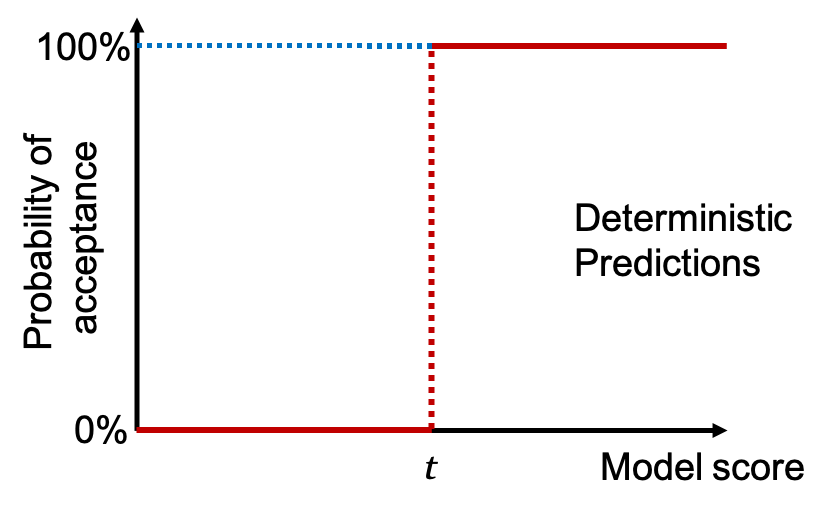
\includegraphics[width=0.6\textwidth]{04_IndividualFairness/figures/Fig_Score2ProbDisc.png}
\caption[Discontinuity in the probability of acceptance as a function of model score.]{Discontinuity in the probability of acceptance as a function of model score (at the threshold $t$) under a deterministic binary classifier.}
\label{fig:DiscThreshold}
\end{figure}

If we want our model to be fair at the individual level, we need to remove the discontinuity (close the gap) at our decision boundary. How might we do this? Let's return to our simple example of the job applicant filter. Let's assume our binary classifier outputs a score and that score is a continuous function of our features. In this case, the discontinuity in our model mapping is a result of the threshold alone because continuity holds under composition. That is to say, a continuous function of a continuous function is also continuous\footnote{More precisely, for $f(x)=g(h(x))$, if $h(x)$ is continuous at $x=a$ and $g(x)$ is continuous at $x=h(a)$ then $f$ is continuous at $x=a$.}. Then if we can remove the discontinuity at the threshold our model mapping will be continuous. Rather than imposing a threshold on the model score and rejecting or accepting individuals based on which side of the threshold they fall, we can use the score to determine the probability of acceptance. We then randomly draw a value according to that probability distribution, to determine if the individual is accepted or not. This approach allows the probability of acceptance to be a continuous function of model score. See for example Figure \ref{fig:ContThreshold}.
%
\begin{figure}[h!]
\centering
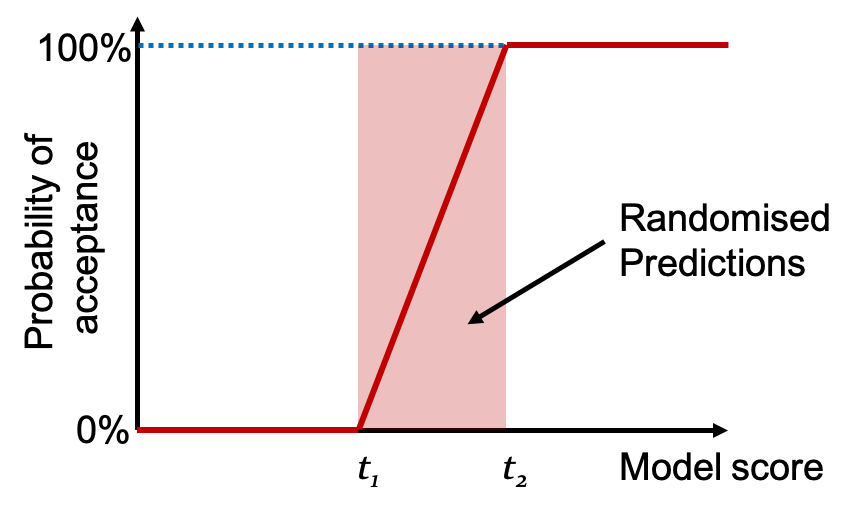
\includegraphics[width=0.6\textwidth]{04_IndividualFairness/figures/Fig_Score2ProbCont.png}
\caption[The probability of acceptance as a function of model score under a randomised binary classifier.]{The probability of acceptance as a function of model score under a randomised binary classifier. The predictions are randomised between thresholds $t_1$ and $t_2$ with the probability of acceptance increasing linearly from zero to one.}
\label{fig:ContThreshold}
\end{figure}

At first glance, this approach might sound a little bizarre. We are saying that in order to remedy the problem, that close to the decision boundary of a classifier similar individuals receive different predictions, we must instead turn to a model which makes a decision at random?! One way of looking at this is opportunity. In a deterministic model we allow arbitrarily similar individuals to be \emph{guaranteed} to receive different predictions. By randomising our predictions we accept that there is uncertainty in our model predictions (especially close to the decision boundary) and our model always gives similar individuals a similar \emph{chance} of being accepted. Note that in Figure \ref{fig:ContThreshold} the predictions are not randomised for all model scores, we have essentially softened our decision boundary by creating a region (between the thresholds $t_1$ and $t_2$) in which model scores result in randomised predictions.

\begin{lookbox}
\lbtitle{Exercise: Randomised predictions}
Write a function which takes the model score from a binary classifier and makes randomised predictions between two thresholds so that the probability of acceptance is a continuous fuction of the model score:
\begin{enumerate}[leftmargin=*]
\item Write a function which maps the model score to the probability of acceptance. The function should take a two thresholds, $t_1<t_2$. The probability of acceptance should be zero if the score is less than $t_1$, one if the score is greater than $t_2$ and increase linearly from zero to one for model scores between the two thresholds.
\item Write a function that takes a probability value $p$ and outputs the value one with probability $p$ and zero with probability $1-p$.
\item Compose the functions above to complete the exercise.
\end{enumerate}
See section 4.5 of the notebook you downloaded and worked through in the previous chapter. \hyperlink{IF_RandPreds}{Solution} in appendix \ref{sec_app_IFSolutions}.
\end{lookbox}

For classification then our model must be probabilistic, that is, it maps each individual in feature space to a distribution over the possible outcomes, which we can then randomly draw from to make predictions. Our predictions are then randomised rather than deterministic and to satisfy individual fairness we require our probabilistic model mapping to be continuous. Let's write our continuity condition for our classifier a little more explicitly.

\begin{lookbox}
\lbtitle{Lipschitz Continuity (Classification)}
Consider our classification model to be a function $f$, which maps individuals $\boldsymbol{x}\in\mathcal{X}$ to distributions $p_{\boldsymbol{x}}(y) \in \mathcal{P}(\mathcal{Y})$ over all possible outcomes $y\in\mathcal{Y}$, that is to say $p_{\boldsymbol{x}}(y)=f(\boldsymbol{x})$ and  $f:\mathcal{X}\mapsto\mathcal{P}(\mathcal{Y})$. Then the mapping $f$ is \emph{Lipschitz continuous} if there exists a real valued, non-negative constant $K \in \Real_{\geq 0}$ such that,
\begin{equation} \label{eq:LipContClf}
d_{\mathcal{P}(\mathcal{Y})}(f(\boldsymbol{x}_i), f(\boldsymbol{x}_j)) \leq K d_{\mathcal{X}}(\boldsymbol{x}_i, \boldsymbol{x}_j) \quad
\forall\,\, \boldsymbol{x}_i, \boldsymbol{x}_j \in \mathcal{X}
\end{equation}
where $d_{\mathcal{X}}:\mathcal{X}\times\mathcal{X}\mapsto\Real$ and $d_{\mathcal{P}(\mathcal{Y})}:\mathcal{P}(\mathcal{Y})\times\mathcal{P}(\mathcal{Y})\mapsto\Real$  denote distance metrics. $d_{\mathcal{X}}$ determines how similar two individuals are in feature space and $d_{\mathcal{P}(\mathcal{Y})}$ measures how similar two probability distributions over $\mathcal{Y}$ are.
\end{lookbox}

Okay, so we have a theoretical understanding of how individual fairness translates to a model behaviour, and that is useful to understand. To summarise, ideally our model mapping is continuous and the smaller the slope of the surface, the more similarly neighbouring individuals are treated. In fact, if the slope is zero everywhere then everyone is treated the same. In this case, all individuals get mapped to the same distribution over outcomes. Of course such a model would not make a very good predictor as it would not take into account the features of the individuals in its predictions. We can then think of the problem of satisfying individual fairness as an additional model requirement. In training our model we want to minimise the total loss on the training data and to satisfy individual fairness we want to bound the model mapping slope to be within some prescribed range $\pm K$.

How might we measure individual fairness? Just as the error of our model will depend on where in feature space we are measuring, so will the slope. The slope, in addition, will also depend on which direction on the model surface we are facing. Any measure of individual fairness which outputs a single value will then be a rather coarse measure. We could simply take the maximum slope between any two data points in the dataset. Alternatively, we could perform an aggregation over the solution surface; one averaging the slope at any given point and another averaging over feature space. Just as we aggregate the loss over a set of data points to get a cost for the model we could aggregate the slope over a set of data points to measure individual fairness.

%%%%%%%%%%%%%%%%%%%%%%%%%%%%%%%%%%%%%%%%%%%%%%%%%%%%%%%%%%%%%%%%%%%%%%%%%%%%
\subsection{Consistency}

The metric consistency, measures individual fairness by looking at the changes in our model output for neighbouring points on a finite set of data points.
\[
yNN = 1 - \frac{1}{n} \sum_{i=1}^n \left| \hat{y}_i -
\frac{1}{k}\sum_{j|x_j\in kNN(\boldsymbol{x}_i)} \hat{y}_j \right|
\]
It is described as measuring ``the consistency of the model classifications locally in input space''\cite{ZemelLearnFairReps}. Values close to one indicate that similar inputs are treated similarly. Note that if all individuals receive the same prediction, consistency will be exactly one.

%%%%%%%%%%%%%%%%%%%%%%%%%%%%%%%%%%%%%%%%%%%%%%%%%%%%%%%%%%%%%%%%%%%%%%%%%%%%
\subsection{Measuring similarity between examples}

A question we have glossed over so far is on the distance metrics. The consistency metric described above, rather conveniently, avoids the need to choose a metric that compares probability distributions over outcomes but we still need a distance metric in feature space to compare how similar two individuals are and thus find the $k$ nearest neighbours. Determining how similar individuals (or more generally examples in feature space) are, is very much a problem that is at the heart of data science and machine learning. It is often answered either explicitly or implicitly by machine learning solutions. How one determines similarity between individuals will depend on the task at hand and a good metric will require domain knowledge.

That said the question of similarity is also clearly related to the question of fairness. To what extent should people be treated the same? What characteristics should we discriminate on the basis of and which ones shouldn't we? And, if we are talking about individual fairness, what does continuity over categorical variables even look like? At the beginning of the chapter we talked about how using different thresholds for male and female candidates in a job applicant filter might conflict with the notion of individual fairness. Then one might think that individual fairness aligns with anti-classification principles, in that if we consider gender to be irrelevant with respect to the task (so that our identical twins, John and Jane from the previous chapter, are the same person according to our distance metric), then individual fairness would prevent us from treating male and female applicants differently. While this may be appropriate for some tasks it need not be the case more generally. We already know that fairness cannot in general be achieved through unawareness. Just as the price of a home in San Francisco might be determined by completely different factors from those of a home in New York City, what if the success in an interview or job is determined by different factors for male and female applicants? If we believe this to be the case then we might reasonably want to use different models for different subgroups of the population. In this scenario, what role does the notion of individual fairness play? In the scenario where, using different models for different subgroups of the population might be more appropriate, there is still value in understanding how consistently each model treats individuals within the subgroups it is applied to.

The user defined distance metric should satisfy the distance metric properties given below to be valid.

%\begin{lookbox}
%\lbtitle{Distance metric properties}
%\begin{wrapfigure}[7]{r}{0.35\textwidth}
%\centering
%\vspace{-1.2cm}
%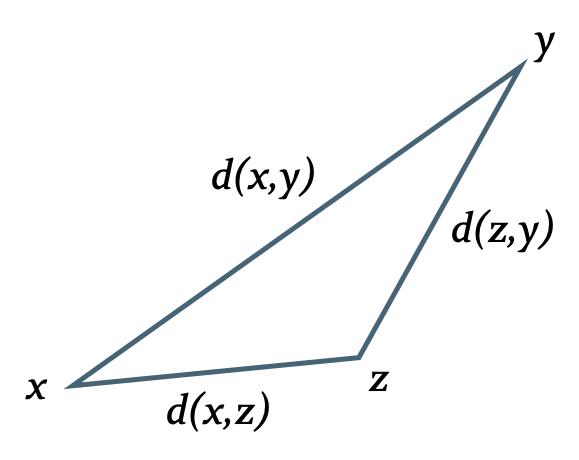
\includegraphics[width=0.3\textwidth]{04_IndividualFairness/figures/Fig_TriangleInequality.png}
%\caption{Triangle inequality.}
%\label{fig:TriIneq}
%\end{wrapfigure}
%A distance metric $d$ on the set $\mathcal{X}$ is a function $d:\mathcal{X}\times\mathcal{X}\mapsto\Real_{\geq 0}$ that has the following properties $\forall\,\,x, y, z\in\mathcal{X}$
%\begin{itemize}
%\item Identity: $d(x,y)=0 \Leftrightarrow x=y$
%\item Symmetry: $d(x,y)=d(y,x)$
%\item Triangle inequality: $d(x,y)\leq d(x,z)+d(z,y)$
%\end{itemize}
%Combining Symmetry with the triangle inequality shows that the metric must return a non-negative value.
%\end{lookbox}
\begin{figure}[h!]
\begin{lookbox}
\begin{minipage}[b]{0.63\textwidth}
\lbtitle{Distance metric properties}
A distance metric $d$ on the set $\mathcal{X}$ is a function $d:\mathcal{X}\times\mathcal{X}\mapsto\Real_{\geq 0}$ that has the following properties $\forall\,\,x, y, z\in\mathcal{X}$
\begin{itemize}
\item Identity: $d(x,y)=0 \Leftrightarrow x=y$
\item Symmetry: $d(x,y)=d(y,x)$
\item Triangle inequality: $d(x,y)\leq d(x,z)+d(z,y)$
\end{itemize}
Combining Symmetry with the triangle inequality shows that the metric must return a non-negative value.
\end{minipage}\hspace{0.05\textwidth}
\begin{minipage}[b]{0.31\textwidth}
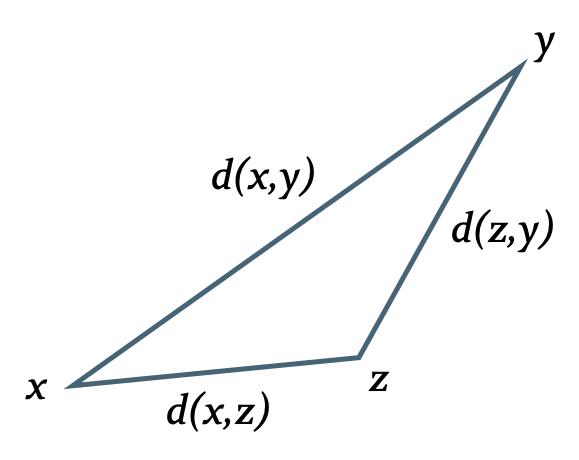
\includegraphics[width=\textwidth]{04_IndividualFairness/figures/Fig_TriangleInequality.png}\vspace{-8pt}
\caption{Triangle inequality.}
\label{fig:TriIneq}
\end{minipage}
\end{lookbox}
\end{figure}\vspace{-\baselineskip}

\noindent The identity property says that the distance between two points is zero if and only if the two points are identical. The symmetry property says that the distance should be independent of the order in which the two points are supplied to the distance function (symmetric with respect to the variables). The triangle inequality says the distance between two points $x$ and $y$ must be less than or equal to the total distance traversed between them via any other given point $z$ (see Figure \ref{fig:TriIneq}).

%%%%%%%%%%%%%%%%%%%%%%%%%%%%%%%%%%%%%%%%%%%%%%%%%%%%%%%%%%%%%%%%%%%%%%%%%%%%
%%%%%%%%%%%%%%%%%%%%%%%%%%%%%%%%%%%%%%%%%%%%%%%%%%%%%%%%%%%%%%%%%%%%%%%%%%%%
\section*{Summary}
\addcontentsline{toc}{section}{Summary}

\begin{itemize}[leftmargin=*]
\item Individual fairness is the idea that a given decision process, is fair if similar people (with respect to the task) receive similar decisions. As a metric, individual fairness cares not about the actual decision, but rather about the consistency with which they are made.
%
\item Individual fairness can be interpreted as a continuity requirement on our data or model. It can broadly be understood as imposing a bound on the slope of our mapping from input (features) to output (predictions or distributions over outcomes).
%
\item A deterministic classifier that outputs a score and then imposes a threshold on it to determine the predicted class cannot satisfy individual fairness by construction, because the threshold results in a discontinuity in the model mapping.
%
\item For a classification model to satisfy individual fairness (continuity) we must turn to a probabilistic model which maps individuals to distributions over outcomes. The continuity requirement then applies to our model mapping. Predictions are then randomised, based on the model output distributions.
%
\item The metric consistency is given by
\[
yNN = 1 - \frac{1}{n} \sum_{i=1}^n \left| \hat{y}_i -
\frac{1}{k}\sum_{j|x_j\in kNN(\boldsymbol{x}_i)} \hat{y}_j \right|.
\]
It uses $k$-Nearest Neighbours to measure the consistency of model classifications locally in input space in an effort to quantify individual fairness in a dataset. Values close to one indicate that similar inputs are treated similarly. 
\end{itemize}

%%%%%%%%%%%%%%%%%%%%%%%%%%%%%%%%%%%%%%%%%%%%%%%%%%%%%%%%%%%%%%%%%%%%%%%%%%%%
\input{99_BackMatter/BibStyle}